\documentclass{llncs}

\usepackage[nocompress]{cite}
\usepackage[english]{babel}
%\usepackage{minted}
\usepackage{array}
\usepackage{url}
\usepackage{ifthen}
\usepackage{graphicx}
\usepackage{amssymb}


%common abbreviations
\newcommand{\etal}{{\it et al.}}
\newcommand{\etc}{{\it etc.}}
\newcommand{\ie}{\emph{i.e.}}
\newcommand{\eg}{{\em e.g.}}

\newboolean{showcomments}
\setboolean{showcomments}{true}

\ifthenelse{\boolean{showcomments}}
{ \newcommand{\mynote}[2]{
    \fbox{\bfseries\sffamily\scriptsize#1}
    {\small$\blacktriangleright$\textsf{\emph{#2}}$\blacktriangleleft$}}}
{\newcommand{\mynote}[2]{}}

\newcommand{\cdu}[1]{\mynote{Corentin}{#1}}
\newcommand{\cd}[1]{\mynote{Charlotte}{#1}}
\newcommand{\sfa}[1]{\mynote{Sabrine}{#1}}
\newcommand{\todo}[1]{\mynote{TODO}{#1}}

\makeatletter
\let\@copyrightspace\relax
\makeatother 

\begin{document}

\title{WAZIUP: An Internet of Things and Big Data platform to boost innovation in Africa}

\author{Charlotte Dupont\inst{1} \and Sabrine Fatnassi\inst{1} \and Corentin Dupont\inst{2}}
\institute{Easy Global Market
Espace Beethoven
1200 Route des lucioles
06560 Valbonne, France\\
\and
Create-Net
via Alla Cascata, 56/D
38123 Trento, Italy\\
\email{{charlotte.dupont,sabrine.fatnassi}@eglobalmark.com}
\email{cdupont@create-net.org}
}

\date{\today}

\maketitle

\begin{abstract}
In this book chapter, we present WAZIUP, a 3 years european project started on February 1st, 2016. 
The aim of the project is to build an open innovation platform to accelerate innovation in Africa through cutting edge IoT effective communications and Big Data Applications. 
As the project is at his beginning, we will give an overview of the project with the description of the IoT and big data platforms such as the technical aspects of implementation and deployement of WAZIUP. 

\end{abstract}


\section{Introduction}

ICT developments in Africa has already enabled significant modernizations across traditional sectors.
Notable examples are the micro-health insurance accessible through mobile devices, index-based crop insurance and crowd-sourced management of public services.
These innovative applications recognize and leverage commonalities between sectors, blur traditional lines, and open up a new field of opportunities.

The opportunity for ICT in Africa is huge especially for IoT and big data: those technologies are promising a big wave of innovation for our daily lives.
The promise of IoT is to connect billions of sensors, devices, equipment and systems.
In turn, the challenge is to drive business outcomes, consumer benefits, and to create new value.
The new mantras for the IoT Era is the collection, convergence and exploitation of data.
The information is collected from sensors, devices, gateways, edge equipment and networks and stored in their respective IoT platforms.
This information is processed in order to increase business efficiency through automation while reducing downtime and improving people productivity.

While developed countries are discussing about massive deployment of IoT, countries in Sub-Saharan Africa are still far from being ready to enjoy the full benefit of Iot.
They face many challenges, such as the lack of infrastructure and the high cost platforms complexity in deployment.
At the same time, it is urgent to promote IoT worldwide : WAZIUP will contribute by reducing part of the technology gap between EU and Africa.
The goal of WAZIUP is to deploy an IoT and big data platform for African needs and validate it through several Sub Saharan Africa real-life use cases.

WAZIUP is a 3 years H2020 international cooperation action started on February 1st, 2016.
The project is driven by a consortium of 5 EU partners and of 7 partners from 4 sub-Saharan African countries.
Furthermore, it has support from multiple African stakeholders with the aim of defining new innovation space to advance the African Rural Economy.
It will do so by involving end-users communities in the loop, namely rural African communities of selected pilots, and by involving relevant public bodies in the project development.
WAZIUP will accelerate innovation in Africa by coupling with current EU innovation in the sector of IoT and Big Data: this EU technology will be specialized to generate African cost effective technologies with an eye to preparing the playground to the future technological waves by solving concrete current needs.
WAZIUP will deliver a communication and big data application platform and generate locally the know how by training by use case and examples.
The use of standards will help to create an interoperable platform, fully open source, oriented to radically new paradigms for innovative application/services delivery.

WAZIUP targets the rural community in Sub-Saharan Africa: about 64\% of the population is living outside cities.
The region will be predominantly rural for at least another generation.
The pace of urbanization here is slower compared to other continents, and the rural population is expected to grow until 2045.
The majority of rural residents live on less than few euros per day.
Rural development is particularly imperative in sub-Saharan Africa, where half of the rural people depends on the agriculture/micro and small farm business, other half faces rare formal employment and pervasive unemployment.
For rural development, technologies have to support several key application sectors such as living quality, health, agriculture and climate changes.

The biggest challenge of WAZIUP is to reduce costs and power consumption while increasing the robustness of the hardware.
Hardware has to be robust enough so as to require lower maintenance and handle environmental and deployment treats as well.
WAZIUP will present an innovative design of the IoT platform dedicated to the rural ecosystem.
To achieve that, low-cost, generic building blocks will be deployed for maximum adaptation to end-applications in the context of the rural economy in developing countries.
Another challenge of WAZIUP is to be able to manage the network deployment and to facilitate IoT communication.
Lower cost solutions has to be used : privilege price and single hop dedicated communication networks, energy autonomous, with low maintenance costs and long lasting operations.
Dynamic management of long range connectivity has to be taken into account (e.g., cope with network \& service fluctuations), such as devices identification, abstraction/virtualization of devices, communication and network resources optimization.
Finally, WAZIUP aim to exploit the potential of big-data applications in the specific rural context.
Data will be collected from the IoT sensors themselves, but WAZIUP will also collect open data from other sources to build predictive models and enrich the platform.

From a technical standpoint, WAZIUP will pay attention to all related privacy and security aspects with specifics addressing the involved communities (farmers, developers).

Applications will receive requirements from users’ needs to have a personalized and friendly interface and will ensure compliance with all most common usability standards\footnote{Web Accessibility Initiative and ISO/TR 16982:2002}.
The platform will be designed through open standard and protocols from the Geospatial Consortium (OGC), W3C, IEEE from the European SDOs (CEN, CENELEC and ETSI) for all its key technology.

Continued Openness will be ensured through the release of open specification and open software components and/or algorithms.
Low-cost and low-energy consumption will be possible through the design of innovation hardware (sensors/actuators), and of IoT communication \& network infrastructure.

The challenges outlined above will be tackled using an open IoT-Big Data Platform with affordable sensors connected through an Iot-Cloud open platform. 
The technical functionalities encompassed by the platform will be a cloud-based real-time data collection combined with analytics and automation software, an intelligent analytics of sensor and device data, an integration to third parties platforms and a Platform-as-a-Service (PaaS) provider. 
The PaaS will provide to business clientele with independently maintained platform upon which their web application, services and mobile applications can be built. 

The rest of this book chapter is structured as follows: Section~\ref{sec:platform} presents the architecture of the WAZIUP platform. 
Section~\ref{sec:implem} shows the implementation chosen. 
Section~\ref{sec:deploy} details the deployement of WAZIUP, contrained by its environment.
Section~\ref{sec:usecases} presents four use cases that will be used to validate the WAZIUP concepts.
Section~\ref{sec:relworks} presents a survey of the literature on the topic, together with a survey of the Big Data Open Source tools.
Finally we conclude the chapter in Section~\ref{sec:conclu}.


\section{IoT \& Big Data Platform}

Challenges of WAZIUP will be tackled using an open IoT-big data platform with affordable sensors connected through an IoT-Cloud open platform.
This platform will also make use of mobile phones and real-time processing to empower users and deliver the needed services.
The project will not develop any new IoT/Big Data software platform, but, rather exploit the existing solutions and adapt them for the purpose. Hereafter a compact list of core technical functionalities encompassed by the platform:

\begin{itemize}
   \item \emph{Cloud-based real-time data collection combined with analytics and automation software:} thus, the platform will offer cost-effective solutions for aggregating different machines and sensor types to engender efficiency, smart automation and optimization in the rural context.
   \item \emph{Intelligent analytics of sensor and device data:} studied in order to optimize for performance of the rural workplace, detect potential outages, and finally reduce overall maintenance costs.
   \item \emph{Integration to 3rd parties' platform:} enables customers' benefit of scaling fast and easy.
   \item \emph{PaaS (Platform-as-a-Service) provider:} WAZIUP will provide to business clientele with independently maintained platform upon which their web application, services and mobile applications can be built.
\end{itemize}

\subsection{Functional overview}
This section presents the functional view of the architecture. 

\begin{figure}[h!]
\centering
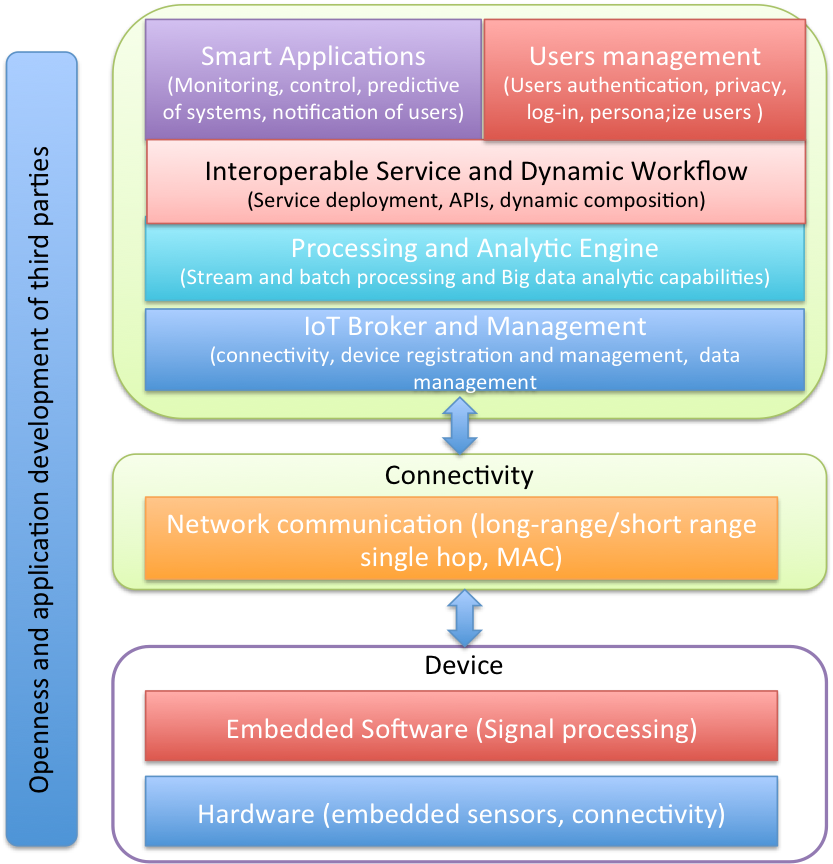
\includegraphics[width=0.7\textwidth]{figs/functional.png}
\caption{Functional overview of WAZIUP}
\label{fig:func}
\end{figure}

The Figure~\ref{fig:func} displays the functional overview of WAZIUP.
The topmost block represents the Cloud platform, the middle one is the network connectivity while the bottom one is the local deployment, including gateway and sensors.
The following functional domains have been identified:

\begin{itemize}
  \item \emph{Application platform}
	Application writing, deploying, hosting and execution.
  \item \emph{Stream and data analytic}
	Data brokering, stream processing and data analytics.
  \item \emph{Users Management}
	Management of the identification, roles and connections of users.
  \item \emph{Gateway, sensors and networks}
	The IoT connectivity, the sensors data and metadata.
  \item \emph{Security and privacy}
	The anonymisation of the data, securisation of the transmissions.
  \item \emph{Platform Management}
	Status of the components, deployment of the platform
\end{itemize}

Based on the functional domains, actors have been identified. 
An actor is either a physical person or an external system. 
There are five actors: the developer, the data provider, the sensor owner, the application user and finally the administrator.

\paragraph{Developer}
The developer uses WAZIUP platform to compile and deploy his application. 
The application is then hosted on the platform and accessible. 
Their tasks are:
\begin{itemize}
	\item \emph{Collect requirements for WAZIUP app}
	\item \emph{Design app architecture}
	\item \emph{Realize app}
	\item \emph{Interact with WAZIUP API}
	\item \emph{Deploy App in WAZIUP PF}
	\item \emph{Maintain app}
\end{itemize}

\paragraph{The data provider}
The data provider is a third party owning an internet API to which WAZIUP is connecting in order to retrieve data. 
Their tasks are:
\begin{itemize}
	\item \emph{Integrate third party API}
	\item \emph{Access control of API}
	\item \emph{Maintain the API}
\end{itemize}

\paragraph{The sensor owner }
The sensor owner is deploying the sensors in the field, and then registering them on the WAZIUP platform. Sensor data then becomes available to applications. Their tasks are:
\begin{itemize}
	\item \emph{Analyze deployment}
	\item \emph{Install sensors}
	\item \emph{Register sensors with WAZIUP}
	\item \emph{Configure sensors }
\end{itemize}

\paragraph{The application user}
The application user is accessing the application developed by the Developer and deployed on WAZIUP. Their tasks are:
\begin{itemize}
	\item \emph{Register with WAZIUP}
	\item \emph{Access/use application}
	\item \emph{Provide feedback on app}
\end{itemize}

\paragraph{The administrator}
The administrator manages and configure the platform; and administrates the users. Their tasks are:
\begin{itemize}
	\item \emph{Manage users accounts}
	\item \emph{Configure the platform}
	\item \emph{Control resources usage}
\end{itemize}

\subsection{IoT platform}

\subsubsection{IoT architecture overview}

WAZIUP IoT platform architecture is presented in Figure~\ref{fig:iotarchi}.
It has three main layers: device layer, gateway layer and the cloud layer.

\begin{figure}[h]
\centering
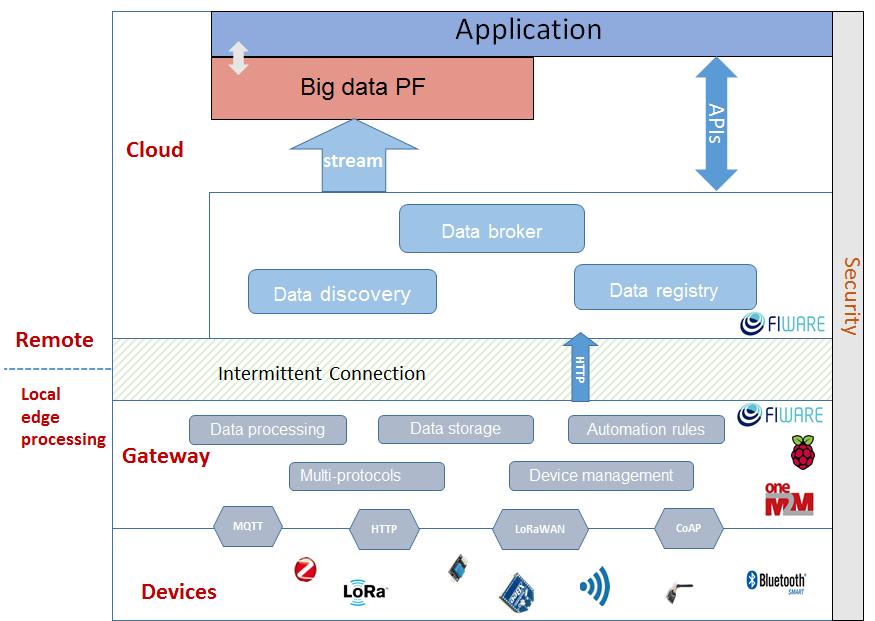
\includegraphics[width=\textwidth]{figs/iotarchi.png}
\caption{IoT platform architecture}
\label{fig:iotarchi}
\end{figure}

\begin{itemize}
  \item \emph{The device layer}
    It includes IoT sensors and actuator that are able to communicate each on its protocol (MQTT, CoAP, HTTP, LoRAWAN) with the gateway. 
It a constraint and autonomous device. 
Considering the project circumstances it has to be low cost and doesn’t consume much power.
  \item \emph{The gateway layer}
  The gateway is a key component in our architecture since it ensure a secure bidirectional communication between the Iot devices and the cloud services.
 It interfere with various kind of devices: getting the data from sensors and sending commands to actuators.
  It has to be multi-protocol in order to be able to support diverse devices and it need to have device management capabilities.
Since the connection is intermittent in our project, it is mandatory that the gateway is able to manage automation rules (for example some event processing), to store data locally and to have low speed internet connectivity (2G: GPRS, EDGE).
  \item \emph{The cloud layer}
  Our cloud main component are: the Data broker, the data registry and the data discovery.
\begin{itemize}
  \item \emph{Data broker:}
    it is the key component of the IoT cloud services, it is based on publish/ subscribe mechanism to ensure data transfer from different producers to their respected consumers.
  \item \emph{Data registry:}
    it contains the virtual representation of devices (the data and the meta-data)
  \item \emph{Data discovery:} 
    it is responsible on querying the data.
\end{itemize}
\end{itemize}

\subsection{Big Data Platform}

The Big Data platform will allow developers to proceed data analysis with cutting-edge tools. 
Based on the state-of-the-art analysis, we will choose the best fitted tools to analyze the data coming from IoT sensors. 
Some specificities will be mandatory, such as the capacity to proceed streaming analysis. 
To make some predictions and to help to decision making, we will need some machine learning capacities, with dedicated algorithms libraries or independant tools.
We will select the Big Data platform analytics tools based on each specific use case which will require different analysis. 
All the tools will be available on the big data platform, to proceed analysis directly on WAZIUP cloud, or to be installed on a local machine, with a manifest to help deploying the analysis.






\section{Implementation}
In this section we will present WAZIUP plateform components and the technology and tools selected for each component.

\subsection{Platform components}
Here is a detailed view of WAZIUP plateforrm components:

\begin{figure}[h!]
\centering
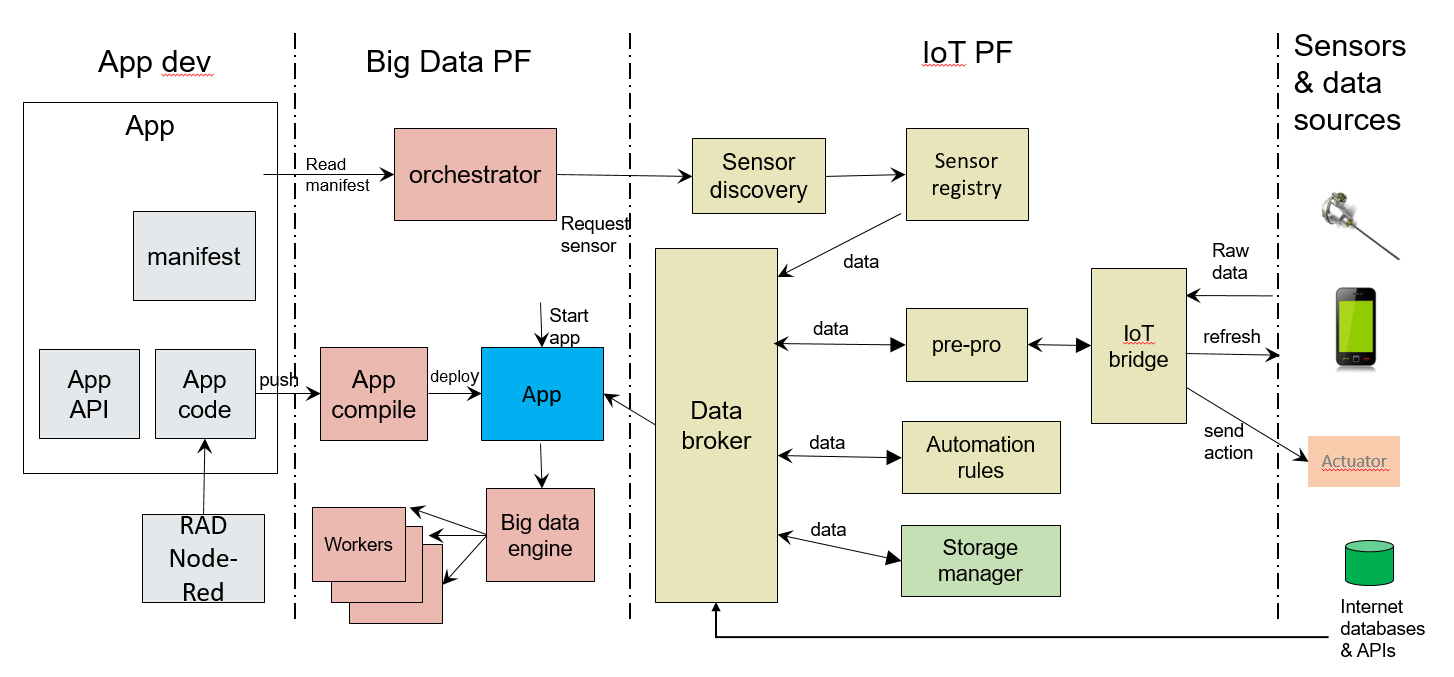
\includegraphics[width=0.9\textwidth]{figs/platformOverview.png}
\caption{WAZIUP IoT platform overview}
\label{fig:platformOverview}
\end{figure}

The figure ~\ref{fig:platformOverview} presents the full WAZIUP architecture. 
There are 4 silos (from left to right): Application development, big data platform, IoT platform, Sensors and data sources. 
The first silo involves the development of the application itself. 
A rapid application development (RAD) tool can be used, such as Node-Red. 
The user provides the code source of the application, together with the manifest. 
The manifest describes the requirements of the application in terms of:
\begin{itemize}
	\item \emph{Compute needs (i.e RAM, CPU, disk)}
	\item \emph{reference to data sources (i.e. sensors, internet - sources...)}
	\item \emph{big data engines needed (i.e Flink, Hadoop...)}
	\item \emph{configuration of sensors (i.e. sampling rate)}
	\item \emph{local and global application deployment}
\end{itemize}

The application source code, together with the manifest, is pushed to the Waziup Cloud platform by the user. 
The orchestrator component will read the manifest and trigger the compilation of the application. 
It will then deploy the application in the Cloud execution environment. 
It will also instantiate the services needed by the application, as described in the manifest. 
The last task of the orchestrator is to request the sensor and data sources connections from the IoT components of the architecture. 
The sensor discovery module will be in charge of retrieving a list of sensors that matches the manifest description.
On the left side of the diagram, the sensor owners can register their sensors with the platform. External data sources such as Internet APIs can also be connected directly to the data broker. 
The sensors selected for each application will deliver their data to the data broker, through the IoT bridge and preprocessor. The IoT bridge is responsible on the senors communication, it receives and transmits data to sensors using its specific protocol. The pre-process can apply transoformation of the received data. The local rule is responsible on executing automated rules. the storage maanger is responsible on storing historic data.

\subsection{Sequence diagrams}
\subsection{Interfaces?}
\subsection{Technology and tools}

In this section we will present the technology choices for each functional component stated above.
In the cloud level the functional component are the data broker, data registry and data discovery.
To cover these functionalities, The FIWARE generic enabler Orion context broker is the all-in-one solution.
It is based on the Next Generic Service Interfaces (NGSI) 9/10.
NGSI specification defines a data model and interfaces to manage the whole cycle of the virtual entities.  
We have also another candidate: the Nec IoT broker that cover the functionality of the data broker and that uses the ConfMan component for the data discovery and registry.
In the gateway level, we have these functionalities:

\begin{itemize}
    \item \emph{Multiprotocol}
The FIWARE IoT agent component: can be an option to ensure this characteristic. 
Each IoT agent can be responsible on the data transfer to and from the devices using the device specific protocol. 
    \item \emph{Device management}
We are considering the use of LwM2M device management protocol.
    \item \emph{Local rules}
FIWARE Cepheus enabler can be an option since it has a complex event processing engine. 
    \item \emph{Data processing}
this component will be developed depending on use cases requirements.
    \item \emph{Data storage}
Mongo DB can be an option, other light data bases can be also considered such as SQLiteDB.
\end{itemize}

In the devices and networking level, LoRa technology captured our attention. 
It specifies LoRaWAN for Low Power Wide Area Network (LPWAN), the kind of technology needed in our project context (rural environment). 
Using LoRaWAN we can reach above 20 km in Line-Of-Sight (LOS) condition between devices and the gateway. 




\section{Deployment}
\label{sec:deploy}

This section will present the innovations of WAZIUP regarding the deployement of the platform.
The first section presents the concept of Platform as a Service adapted to IoT, while the second shows how the concept of local Cloud is essential in African context.

\subsection{PaaS for IoT}

Platform as a Service is a category of cloud computing service that provides a platform allowing customers to develop, run, and manage applications without the complexity of building and maintaining the infrastructure typically associated with developing and deploying an application.
Typically, a PaaS framework will compile an application from its source code, and then deploy it inside lightweight virtual machines, or containers.This compilation and deployment is done with the help of a file called the manifest, which allows the developer to describe the configuration and resource needs for his application.
The manifest file will also describe the services that the application requires and that the platform will need to provision.
Furthermore, PaaS environments usually offer an interface to scale up or down applications, or to schedule various tasks within the applications.

The idea of WAZIUP is to extend the paradigm of the PaaS to IoT.
Developing an IoT Big data application is a complex task.
A lot of services need to be installed and configured, such as databases and complex event processing engines.
Furthermore, it requires an advanced knowledge of the various communication protocols, the programming of embedded devices, the storage, processing and analysis of the data in a distributed fashion and finally the programming of GUIs and user interactions.
The promise of the PaaS extended to IoT is to abstract away this work to a large extent.

\begin{figure}[h!]
\centering
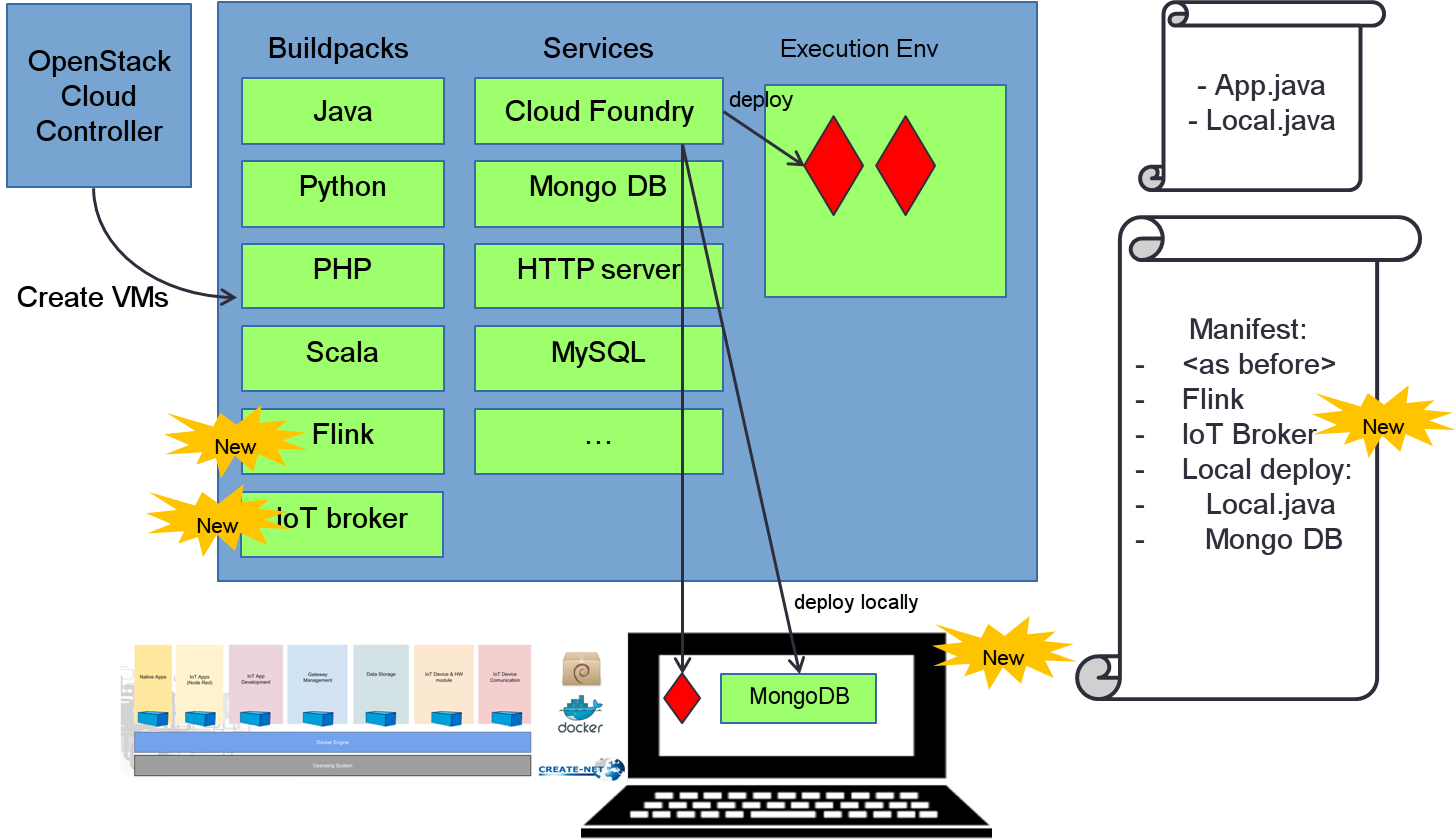
\includegraphics[width=0.7\textwidth]{figs/paas.png}
\caption{PaaS deployment extended for IoT}
\label{fig:paas}
\end{figure}

The Figure~\ref{fig:paas} shows the PaaS deployment in WAZIUP.
Traditional PaaS environment are usually installed on top of IaaS (in blue in the picture).
The blue boxes are physical servers, respectively the Cloud Controller and one Compute node.
The PaaS environment is then installed inside the IaaS VMs, in green in the picture.
We use Cloud Foundry as a PaaS framework.
It comes with a certain number of build packs, which and programming languages compilers and run time environments.
It also provides a certain number of preinstalled services such as MongoDB or Apache Tomcat.
The manifest file, showed on the right hand side, provide a high-level language that allows describing which services to instantiate.
We propose to extend this language to IoT and big data services:
\begin{itemize}
  \item Data stream and message broker
  \item CEP engines
  \item Batch processing engines
  \item Data visualization engines
\end{itemize}

Furthermore, we propose to include in the manifest a description of the IoT sensors that are required by the application.
This query includes data such as the sensor type, location and owner.
The manifest also includes the configuration of the sensors.
The application will then be deployed both in the global Cloud and in the local Cloud.

\subsection{Local and global Clouds}

An important feature in WAZIUP platform deployment is the possibility to have a local cloud platform. 
It  is an infrastructure able to deliver services to clients in a limited geographical area. 
The local Cloud replicates some of the features provided by the traditional Cloud. 
It is used for clients that doesn't have a good access to the traditional Cloud, or to provide additional processing power to local services. 
In order for such an infrastructure to be considered as a Local Cloud it must support a virtualization technology. 
In the case of WAZIUP, the local Cloud comprises the end user or service provider PC and IoT Gateway. 
The local Cloud characteristics are:

\begin{itemize}
    \item Existence of IoT devices attached
    \item Can have geographical characteristics
    \item Must support virtualization
    \item Must support local cloud components
    \item Has an identifiable administrator/owner
    \item Has certain regulations/privacy considerations for data access and treatment
\end{itemize}

The Global Cloud, on the other end, is a “backbone infrastructure” which increases the business opportunities for service providers and allows services to access a virtually infinite amount of computing resources. 
In order for such an infrastructure to be considered as a Global Cloud it must support a virtualization technology and be able to host the global cloud components of the WAZIUP architecture.
The figure below present our deployment vision of WAZIUP platform:

\begin{figure}[h!]
\centering
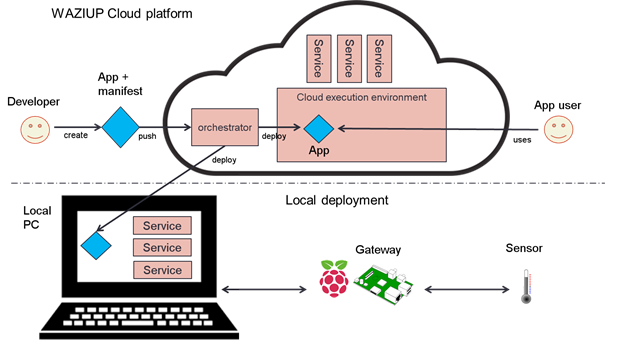
\includegraphics[width=0.7\textwidth]{figs/deploy.png}
\caption{WAZIUP deployment overview}
\label{fig:deploy}
\end{figure}

The Figure~\ref{fig:func} displays the WAZIUP deployment overview.

On the left hand side of the picture, the application is designed by the developer, together with the manifest file. 
It is pushed on the Waziup Cloud platform. The orchestrator then takes care of compiling and deploying the application in the various Cloud execution environments. 
Furthermore, the orchestrator drives the instantiation of the services in the Cloud, according to the manifest. 
The manifest is also describing which part of the application need to be installed locally, together with corresponding services. 
The local application can then connect to the gateway and collect data from the sensors.
The code will be deployed at gateway level, in a similar way than resin.io\footnote{http://resin.io}.




\section{Use case applications}
\label{sec:usecases}

The project will build a strong community able to address innovation in the African rural ecosystem through EU ICT technology.
Actors from various disciplines, including those having industrial backgrounds, those from application areas and target end-users will push towards the creation of an African-European innovation ecosystems based on the open sources for the IoT-Big data platform.
Starting from the rural domain, the project technology will allow the
African young application developer to produce new added value supporting multiple applications domains in the long run.
The induced ecosystem renews the business paradigm: new benefits are engendered from providing and sharing devices, services, and data across stakeholders and applications.

\subsection{Fish farming}

Two different test bed scenarios will be used to effectively integrate the real world fish farming situations/solutions with the digital world of WAZIUP.
The first test-bed is located in a small farm with 4 mini ponds of 90*90 metres and a large farm which operate several ponds of different sizes\footnote{http://www.kumahfarms.com/}.
These two farms produces both tilapia and catfish.
This use case validation will deploy sensor nodes responsible for sensing three parameters from the fish ponds: dissolved oxigen level, temperature and Ph.
The sensor nodes will communicate with the gateways which stores the data locally.
If the internet is available through Wifi of GPRS/UMTS, the data will be send to the Cloud instance of Waziup.

\subsection{Cattle breeding}

With the collaboration of the surrounding farmers we will put sensors around the cows’ neck in order to have measure related to location and speed.
We can also work with CIMEL(Centre d’Impulsion et de Modernisations de l’ELevage) which is a public structure for livestock impulsion and modernisation.
With this center we can make test and simulate a cattle rustling case.
To make this more interesting we imagine a smart food distribution system on CIMEL for a more optimal management of farmers’ ressources.

\subsection{Crop farming}

Weather surely plays a crucial role during the crop growth seasons.
Severe weather can impact crop growth by affecting different bio-physiological processes.
The impact on crop growth depends on the nature of extreme weather event, the crop type and time when it occurs.
Detrimental impact of extreme weather events may be alleviated by taking timely and appropriate preventive measures to cope with the nature and intensity of these weather events.
The availability of local weather predictions is a key factor in the decision process of the farmers.
For example, inputs that are added in the field (such as fertilizer of pesticides) can be lost if rain comes in the next few hours.
This use case presents how the WAZIUP platform can be used to prevent and alleviate the risks due to weather in farms.
To validate this use case, the WAZIUP project will build a low-cost weather station based on Arduino.
The data collected will be processed by the WAZIUP platform and will serve to adjust weather predictions on a local level.

For the deployment of the test bed, two pilots will be conducted in Ghana and Burkina Faso.
Both experimental farmer at the university and operational farm environment will be used as test-beds.
They will provide the possibility to interact directly with farmers, professionals and students who work on these farms.

\subsection{Supply chain management}

Transport is a key point of development for Africa.
It is very important, for food safety and delivery efficiency, to be able to track the origin and transportation of goods.
The test bed will consist of the deployement of a good tracking system.
For the sake of simplicity, the system will be based on SMS.
SMS is the communication platform that is the most available across African countries, even in remote areas.
The system will allow the operators to update the status of the delivery, sending SMS keywords such as "In transit", "Delivered".
The client will be updated on the delivery date and location.
The client will also be able to interact with the system, for example to change the delivery location.





\section{Related works}


\subsection{Review of literature}

In~\cite{Bing2012}, the author presents...

\subsection{Review of Big Data tools}

Far from an exhaustive list, this paragraph describes the most used Open Source Big Data tools and compares them in order to give a better understanding of the Big Data ecosystem. Moreover, this review gives an indication on the best tools fitted for WAZIUP platform. 


\paragraph{Databases and data warehouses}

HDFS, developed by Apache, is a distributed, scalable and portable file-system written in Java for the Hadoop Framework\footnote{https://hadoop.apache.org/docs/r1.2.1/hdfs\_design.html}.
It has been designed for large dataset analysis and by its structure has high fault tolerance. It is the basis upon which everything works in the Hadoop Ecosystem.
Build on top of HDFS, Apache HBase is a distributed, non-relational column oriented datastore\footnote{https://hbase.apache.org/}.
HBase is designed to efficiently address random access and fast record lookup.
It has the capability to handle extremely large tables of data with low latency.
Though, this data storage tool should be used when random and real-time read/write access to data is needed and when many thousands of operation per seconds need to be performed on large datasets (up to petabytes).

Apache Hive\footnote{https://hive.apache.org/} is a data warehouse infrastructure that can manage and query unstructured data as if it were structured.
As a full component of Hadoop Ecosystem, it uses MapReduce for execution and HDFS for storage.
It has its own language SQL-like (HiveQL) that brings expressiveness to the queries.
This storage mode should be used for SQL-like queries and when higher language than MapReduce is needed.
Used by big companies who can’t afford to lose data (Apple, Netflix, Spotify …)(ref), Apache Cassandra is a column oriented database of structured data. The data are highly available thru column indexes and are automatically replicated thru multiple nodes for fault tolerance (ref).
Cassandra has a unique masterless “ring” design that is easy to setup and to maintain (ref).This tools should be use when losing data is not the critical point and not affordable.  

First considered as an outsider, getting rid of traditional table-based relational database, mongoDB quickly became a must-have tool: a NoSQL, relational, document oriented database (ref).
Document are shared in JSON format with dynamic schemas (called BSON) and makes the integration of data sometimes easier.
This database is very useful when you need to consume your data in many applications, as many connectors have been developed.

\paragraph{Data publication and subscription}

Apache Flume is a distributed, reliable and available service for efficiently collecting, aggregating and moving large amounts of streaming event data (ref).
Flume should be used if the data is designed for Hadoop as it can move them to HDFS.
It has many built-in sources and sinks and can process data in-flight using interceptors, which is useful for data masking or filtering.
It is composed of agents and data collectors (and interceptors if needed).

More general purpose, Apache Kafka is a high-throughput, distributed, publish-subscribe messaging system (ref).
It can replicate events, has low latency and is capable of data partitioning. Kafka is also easily scalable and this tool is very useful when the data is to be consumed by multiple applications. It is composed of producer, consumers and topics.
Actually, we might not have to choose between Kafka and Flume, as both can work quite well together.
If the workflow design requires streaming data from Kafka to Hadoop, using a Flume agent with Kafka source to read the data makes sense.
This association is quite common and is called Flafka (ref).

If a Data/Context Scenario is developed, we may need to use a context broker.
Orion Context Broker (FIWARE platform) is a publish/subscribe platform that is able to register context elements and manage them through updates and queries (ref).
It is possible to subscribe to context information when some conditions occurs (e.g. an interval of time passed or the context elements have changed).
Orion is a C++ implementation of the NGSI9/10 REST API binding developed as a part of the FIWARE platform.

\paragraph{Data processing}

Obviously, choosing a data processing tool depends mostly on the outcome expected from the data.
The most common tool for BigData analysis, and what we probably think at first, is Hadoop MapReduce.
It has proven its efficiency in many ways and is an incredible tool.
But if we want to step a bit aside of Hadoop workflow or if we have specific needs, other tools exists and some are becoming more and more powerful.

But first, let’s talk about this milestone Hadoop MapReduce.
MapReduce programming model contributed to the amazing progress of BigData processing this past decade (ref).
By breaking down the work and recombining it in series of parallelizable operations, it is simple but incredibly efficient and scalable to ten thousands of machines if needed.
It can run on inexpensive hardware, lowering the cost of a computing cluster.
The latest version of MapReduce is YARN, called also MapReduce 2.0.

If a higher level of programming on top of MapReduce is needed, Apache Pig is the one.
Pig has its own language (PigLatin) similar to SQL and works on top of MapReduce (ref).
Pig Engine parses, optimizes and automatically executes PigLatin scripts as a series of MapReduce jobs on a Hadoop cluster.
It’s easy to learn and opens Hadoop to data professionals who may not be software engineers.

First designed to work with HDFS on top of YARN (ref), Apache Spark is a different system for processing data and can work out of Hadoop ecosystem with other data managements systems.
It does not work with MapReduce and it can be up to a hundred times faster than MapReduce with its capacity to work in-memory, allowing to keep large working datasets in-memory between jobs, reducing considerably the latency (ref).
What makes it more and more attractive to many users worldwide, is its wide range of applications: batch and stream processing (micro-batch processing with 0.5s latency), machine learning (MLib), SQL (with Hive), graph Analytics (graphX).
Language supported are Java, Python and Scala.

Demand for stream processing becoming more and more important in Big Data analysis, Apache Flink has been recently developed (ref) and is growing very fast.
Flink is a streaming dataflow engine that provides data distribution, communication and fault tolerance.
It has almost no latency as the data are streamed in real-time (row by row).
It runs on YARN and works with its own extended version of MapReduce. Language supported are Java and Scala.

\paragraph{Machine learning}

Machine learning is the union between statistics and artificial intelligence.
It blends AI heuristics with advanced statistical analysis.
We let the machine learn about the data, make decisions, and then apply statistics (ref).
Algorithms used for this tasks can be grouped in 3 domains of actions: Classification, association and clustering (ref).
To choose an algorithm, different parameters must be considered: scalability, robustness, transparency and proportionality.
Overlearning (or overfitting) of the model must be carefully checked.

Without any math or programming requirement, KNIME is an analytic platform that allow the user to proceed the data in a user-friendly graphical interface (ref).
It is a good tool to train your model and evaluate different machine learning algorithms rapidly.
If the workflow is already deployed on Hadoop, a machine learning library exists and is called Mahout (ref).
Spark also has his own machine learning library called MLib (ref).
H20 is a software dedicated to machine-learning, which can be deployed on Hadoop or Spark (Flink in development) (ref).
It has an easy to use Web interface, which makes possible to combine big data analytics easily with machine learning algorithm to train models.

\paragraph{Data visualisation and exploration}

To visualise the data in real time, Freeboard provides a simple, real-time dashboard, commonly used in IoT world (ref).
There is a direct Orion Fiware connector (ref).
To connect with streaming engines, a JSON connector can be used.
Design is simple and customisation is not possible, but it is a very good dashboard to visualise easily raw data coming from sensors, before data analysis.

Tableau Public offers a good visualisation and exploration tool on batch data.
Tableau is a software where you can upload your analysed data (previously extracted in .csv format).
The visualisation tool is very powerful and allow a deep exploration the data.
However it is not designed for really Big Data with large datasets and the open Source version of Tableau (Public) does not offer the data streaming capacities (e.g. Spark connectors).
Nevertheless, Tableau Public is a highly customisable, user-friendly and intuitive exploration tool for data that have already been processed and analysed.

To visualise data in real-time, after analysis (filtering, aggregating, correlating …), one of the best tool is probably Kibana (ref).
It is the visualisation tool coming with ElasticSearch.
Elasticsearch is a search server based on Apache Lucene that provides a distributed, multitenant-capable full-text search engine with an HTTP web interface and schema-free JSON documents (ref).
It is really designed for real-time analytics, most commonly used with Flink or Spark Streaming.



\section{Conclusion}
With ICT technologies, Africa can dramatically improve its agricultural productivity by enabling the muchmore rapid and cost-effective deployment of advanced and real time monitoring and evaluation applications and systems. 
The immediate effect is to improve coordination and logistics, by reducing time and investment horizons for Research and Development and new product development, and by allowing for the enhanced analysis of historical and ongoing data. 
With respect to the water sector, such systems can also dramatically improve water use efficiency, allow for the growth of water provider SMEs by providing practical and cost effective new payment, monitoring and management systems.
This technology can also offer a new cost-effective alternative for integrated watershed management by networking real-time water quality and flow data. 
Furthermore, given the fundamental roles which agriculture and water play in the African economic and social development and more generally onto environmental sustainability, WAZIUP can both directly and indirectly bring a much wider range of benefits related to food security, gender equality, poverty reduction and resource use efficiency.


\section*{Acknowledgements}

This work has been carried out within the European project WAZIUP (H2020-ICT-687607).



\bibliographystyle{unsrt}
\bibliography{central-bibliography/bibliography}

\end{document}
